\documentclass[mathserif]{beamer}
\mode<presentation>
{
  \usetheme{Frankfurt}
  \setbeamercovered{transparent}
}

\setbeamertemplate{caption}[numbered]

\usepackage{bm}
\usefonttheme[onlymath]{serif}
\usepackage{mathrsfs}

\begin{document}


\title{Understanding Deep Learning Requires Rethinking Generalization}

\author{Wenhao Yang
}
\institute{School of Mathematical Sciences

Peking University}
\begin{frame}
  \titlepage
\end{frame}

\date{}

\begin{frame}{Outline}
\tableofcontents
\end{frame}

\section{Deep neural networks easily fit random labels}
\begin{frame}[t]{Fitting Random Labels and Pixels}
  \begin{itemize}
  \item \textbf{True labels: }the original dataset without modification.
  \item \textbf{Partially corrupted labels: }independently with probability $p$,
  the label of each image is corrupted as a uniform random class.
  \item \textbf{Random labels: }all the labels are replaced with random ones.
  \item \textbf{Shuffled pixels: }a random permutation of the pixels is chosen
  and then the same permutation is applied to all the images in both training
  and test section
  \item \textbf{Random pixels: }a different random permutation is applied to
  each image independently.
  \item \textbf{Gaussian: }A Gaussian distribution(with matching mean and
  variance to the original image dataset) is used to generate random
  pixels for each image.
\end{itemize}
\end{frame}
%--- Next Frame ---%
\begin{frame}[t]{Fitting Random easily fit random labels}
  \begin{figure}
    \centering
    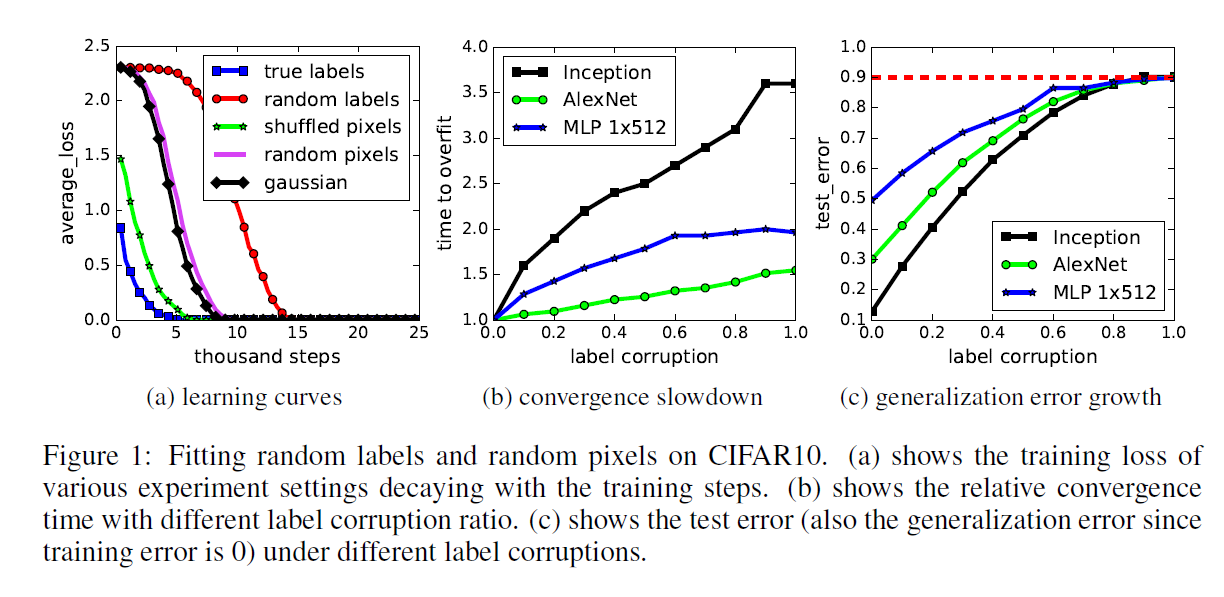
\includegraphics[scale=0.5]{fig/1}
  \end{figure}
\end{frame}

\section{Explicit Regularization}
\begin{frame}[t]{The Role of Explicit Regularization}
\begin{itemize}
  \item Explicit regularization may improve generalization performance,
  but is neither necessary nor by itself sufficient for controlling
  generalization error.
  \item \textbf{Data augmentation: }augment the training set via domain-
  specific transformations. For image data, commonly used transformations
  include random cropping, random perturbation of brightness, saturation,
  hue and contrast.
  \item \textbf{Weight decay: }equivalent to a $l_{2}$ regularizer on the
  weights; also equivalent to a hard constrain of the weights to an
  Euclidean ball, with the radius decided by the amout of weight decay.
  \item \textbf{Dropout: }Mask out each element of a layer output randomly
  with a given dropout probability. Only the Inception V3 for ImageNet uses
  dropout in our experiments.
\end{itemize}
\end{frame}

\begin{frame}[t]{The Role of Explicit Regularization}
  \begin{figure}
    \centering
    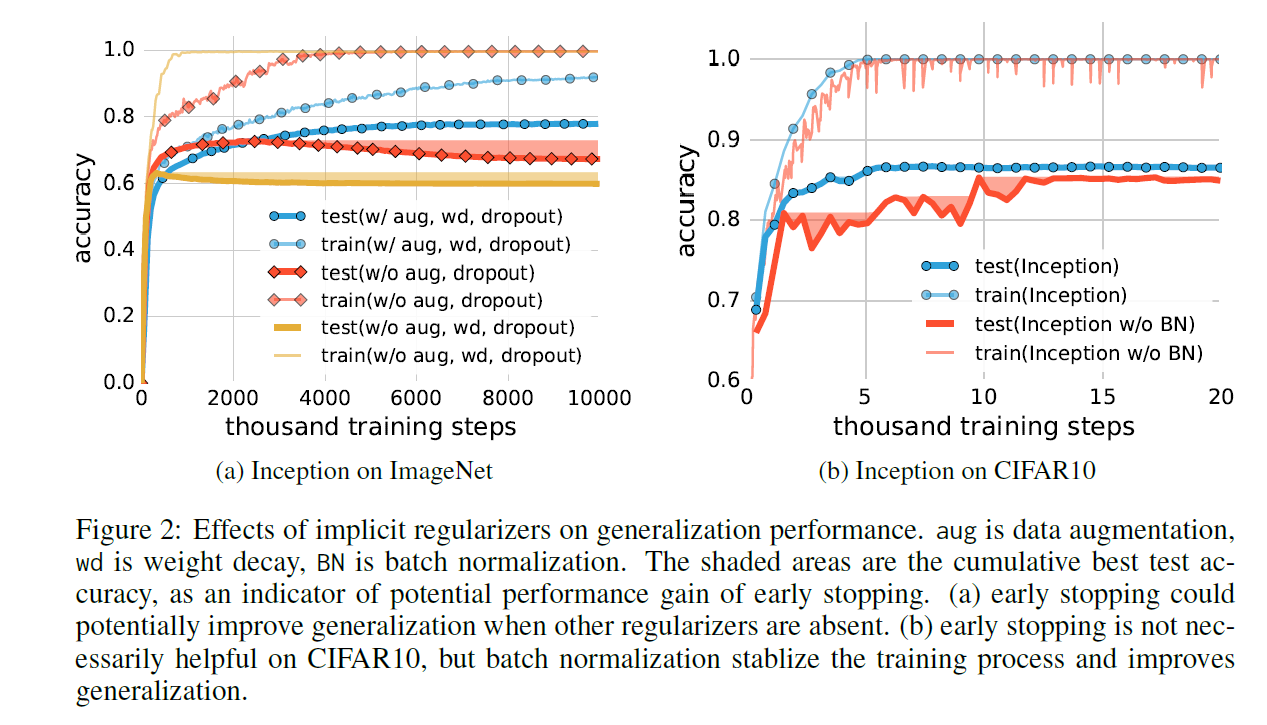
\includegraphics[scale=0.5]{fig/2}
  \end{figure}
\end{frame}

\section{Finite Sample Expressivity}
\begin{frame}[t]{Finite Sample Expressivity}
  \begin{itemize}
    \item Generically large neural networks can express any labeling of
    the training data.
    \item E.g. A simple 2-layer ReLU network with $p=2n+d$ parameters
    can express any labeling of any sample of size $n$ in $d$ dimensions:
    For weight $w,b\in R^{n}$ and $a\in R^{d}$,consider the function:
    \begin{align}
      c(x)=\sum_{j=1}^{n}w_{j}\max\{<a,x>-b_{j},0\}
    \end{align}
    Fix sample $z_{1},..,z_{n}$,and target $y_{1},..,y_{n}$,find $a,b$
    that satisfies $x_{i}=<a,z_{i}>$ and $b_{1}<x_{1}<b_{2}<...<b_{n}<x_{n}$.
    And find $w$ that satisfies $y=Aw$ as $A$ is a full rank matrix, where
    $A_{ij}=\max\{x_{i}-b_{j},0\}$
  \end{itemize}
\end{frame}
\section{Implicit Regularization}
\begin{frame}[t]{The Role of Implicit Regularization}
  \begin{itemize}
    \item Blackboard
  \end{itemize}
\end{frame}

\section{Reference}
\begin{frame}{Reference}
  Reference:

  [1] Chiyuan Zhang, Samy Bengio, Moritz Hardt, Benjamin Recht, Oriol Vinyals; Understanding deep learning requires rethinking generalization
\end{frame}
\end{document}
